% Options for packages loaded elsewhere
\PassOptionsToPackage{unicode}{hyperref}
\PassOptionsToPackage{hyphens}{url}
%
\documentclass[
]{article}
\usepackage{amsmath,amssymb}
\usepackage{lmodern}
\usepackage{iftex}
\ifPDFTeX
  \usepackage[T1]{fontenc}
  \usepackage[utf8]{inputenc}
  \usepackage{textcomp} % provide euro and other symbols
\else % if luatex or xetex
  \usepackage{unicode-math}
  \defaultfontfeatures{Scale=MatchLowercase}
  \defaultfontfeatures[\rmfamily]{Ligatures=TeX,Scale=1}
\fi
% Use upquote if available, for straight quotes in verbatim environments
\IfFileExists{upquote.sty}{\usepackage{upquote}}{}
\IfFileExists{microtype.sty}{% use microtype if available
  \usepackage[]{microtype}
  \UseMicrotypeSet[protrusion]{basicmath} % disable protrusion for tt fonts
}{}
\makeatletter
\@ifundefined{KOMAClassName}{% if non-KOMA class
  \IfFileExists{parskip.sty}{%
    \usepackage{parskip}
  }{% else
    \setlength{\parindent}{0pt}
    \setlength{\parskip}{6pt plus 2pt minus 1pt}}
}{% if KOMA class
  \KOMAoptions{parskip=half}}
\makeatother
\usepackage{xcolor}
\IfFileExists{xurl.sty}{\usepackage{xurl}}{} % add URL line breaks if available
\IfFileExists{bookmark.sty}{\usepackage{bookmark}}{\usepackage{hyperref}}
\hypersetup{
  pdftitle={Untitled},
  hidelinks,
  pdfcreator={LaTeX via pandoc}}
\urlstyle{same} % disable monospaced font for URLs
\usepackage[margin=1in]{geometry}
\usepackage{color}
\usepackage{fancyvrb}
\newcommand{\VerbBar}{|}
\newcommand{\VERB}{\Verb[commandchars=\\\{\}]}
\DefineVerbatimEnvironment{Highlighting}{Verbatim}{commandchars=\\\{\}}
% Add ',fontsize=\small' for more characters per line
\usepackage{framed}
\definecolor{shadecolor}{RGB}{248,248,248}
\newenvironment{Shaded}{\begin{snugshade}}{\end{snugshade}}
\newcommand{\AlertTok}[1]{\textcolor[rgb]{0.94,0.16,0.16}{#1}}
\newcommand{\AnnotationTok}[1]{\textcolor[rgb]{0.56,0.35,0.01}{\textbf{\textit{#1}}}}
\newcommand{\AttributeTok}[1]{\textcolor[rgb]{0.77,0.63,0.00}{#1}}
\newcommand{\BaseNTok}[1]{\textcolor[rgb]{0.00,0.00,0.81}{#1}}
\newcommand{\BuiltInTok}[1]{#1}
\newcommand{\CharTok}[1]{\textcolor[rgb]{0.31,0.60,0.02}{#1}}
\newcommand{\CommentTok}[1]{\textcolor[rgb]{0.56,0.35,0.01}{\textit{#1}}}
\newcommand{\CommentVarTok}[1]{\textcolor[rgb]{0.56,0.35,0.01}{\textbf{\textit{#1}}}}
\newcommand{\ConstantTok}[1]{\textcolor[rgb]{0.00,0.00,0.00}{#1}}
\newcommand{\ControlFlowTok}[1]{\textcolor[rgb]{0.13,0.29,0.53}{\textbf{#1}}}
\newcommand{\DataTypeTok}[1]{\textcolor[rgb]{0.13,0.29,0.53}{#1}}
\newcommand{\DecValTok}[1]{\textcolor[rgb]{0.00,0.00,0.81}{#1}}
\newcommand{\DocumentationTok}[1]{\textcolor[rgb]{0.56,0.35,0.01}{\textbf{\textit{#1}}}}
\newcommand{\ErrorTok}[1]{\textcolor[rgb]{0.64,0.00,0.00}{\textbf{#1}}}
\newcommand{\ExtensionTok}[1]{#1}
\newcommand{\FloatTok}[1]{\textcolor[rgb]{0.00,0.00,0.81}{#1}}
\newcommand{\FunctionTok}[1]{\textcolor[rgb]{0.00,0.00,0.00}{#1}}
\newcommand{\ImportTok}[1]{#1}
\newcommand{\InformationTok}[1]{\textcolor[rgb]{0.56,0.35,0.01}{\textbf{\textit{#1}}}}
\newcommand{\KeywordTok}[1]{\textcolor[rgb]{0.13,0.29,0.53}{\textbf{#1}}}
\newcommand{\NormalTok}[1]{#1}
\newcommand{\OperatorTok}[1]{\textcolor[rgb]{0.81,0.36,0.00}{\textbf{#1}}}
\newcommand{\OtherTok}[1]{\textcolor[rgb]{0.56,0.35,0.01}{#1}}
\newcommand{\PreprocessorTok}[1]{\textcolor[rgb]{0.56,0.35,0.01}{\textit{#1}}}
\newcommand{\RegionMarkerTok}[1]{#1}
\newcommand{\SpecialCharTok}[1]{\textcolor[rgb]{0.00,0.00,0.00}{#1}}
\newcommand{\SpecialStringTok}[1]{\textcolor[rgb]{0.31,0.60,0.02}{#1}}
\newcommand{\StringTok}[1]{\textcolor[rgb]{0.31,0.60,0.02}{#1}}
\newcommand{\VariableTok}[1]{\textcolor[rgb]{0.00,0.00,0.00}{#1}}
\newcommand{\VerbatimStringTok}[1]{\textcolor[rgb]{0.31,0.60,0.02}{#1}}
\newcommand{\WarningTok}[1]{\textcolor[rgb]{0.56,0.35,0.01}{\textbf{\textit{#1}}}}
\usepackage{longtable,booktabs,array}
\usepackage{calc} % for calculating minipage widths
% Correct order of tables after \paragraph or \subparagraph
\usepackage{etoolbox}
\makeatletter
\patchcmd\longtable{\par}{\if@noskipsec\mbox{}\fi\par}{}{}
\makeatother
% Allow footnotes in longtable head/foot
\IfFileExists{footnotehyper.sty}{\usepackage{footnotehyper}}{\usepackage{footnote}}
\makesavenoteenv{longtable}
\usepackage{graphicx}
\makeatletter
\def\maxwidth{\ifdim\Gin@nat@width>\linewidth\linewidth\else\Gin@nat@width\fi}
\def\maxheight{\ifdim\Gin@nat@height>\textheight\textheight\else\Gin@nat@height\fi}
\makeatother
% Scale images if necessary, so that they will not overflow the page
% margins by default, and it is still possible to overwrite the defaults
% using explicit options in \includegraphics[width, height, ...]{}
\setkeys{Gin}{width=\maxwidth,height=\maxheight,keepaspectratio}
% Set default figure placement to htbp
\makeatletter
\def\fps@figure{htbp}
\makeatother
\setlength{\emergencystretch}{3em} % prevent overfull lines
\providecommand{\tightlist}{%
  \setlength{\itemsep}{0pt}\setlength{\parskip}{0pt}}
\setcounter{secnumdepth}{5}
\usepackage{subfig}
\ifLuaTeX
  \usepackage{selnolig}  % disable illegal ligatures
\fi

\title{Untitled}
\author{}
\date{\vspace{-2.5em}2022-06-11}

\begin{document}
\maketitle

{
\setcounter{tocdepth}{2}
\tableofcontents
}
\hypertarget{r-markdown}{%
\subsection{R Markdown}\label{r-markdown}}

\begin{Shaded}
\begin{Highlighting}[]
\NormalTok{EViews\textgreater{} wfcreate(wf=sagiru,page=mati) q 2000 2025}
\NormalTok{+ for \%y page1 page2 page3 page4}
\NormalTok{+ pagecreate(page=\{\%y\}) q 2000 2025}
\NormalTok{+ next}
\NormalTok{+ \%pagelist=@pagelist}
\NormalTok{+ \textquotesingle{}open mychunk}
\NormalTok{+ for \%y \{\%pagelist\}}
\NormalTok{+ pageselect \{\%y\}}
\NormalTok{+ delete gra*}
\NormalTok{+ genr y=@cumsum(nrnd)}
\NormalTok{+ genr x=@cumsum(nrnd)}
\NormalTok{+ genr z=@cumsum(nrnd)}
\NormalTok{+ genr date=@date}
\NormalTok{+                      graph grap1.line z  }
\NormalTok{+                            graph grap2.line z y x}
\NormalTok{+    freeze(grap,mode=overwrite) x.line}
\NormalTok{+ equation ols.ls y c x}
\NormalTok{+ next}
\NormalTok{+ wfsave mychunk}
\end{Highlighting}
\end{Shaded}

\begin{figure}[h]

{\centering \subfloat[A figure\label{fig:mychunk-1}]{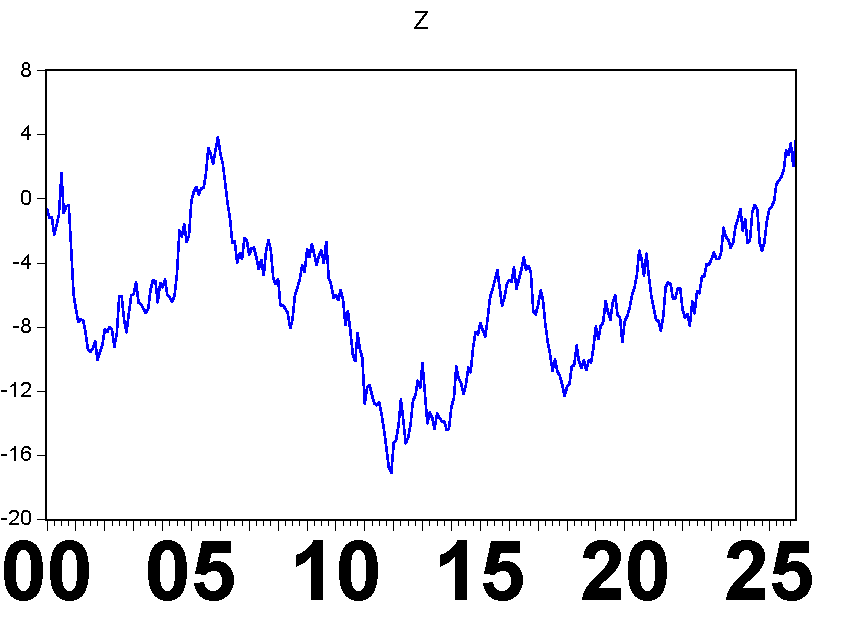
\includegraphics[width=0.45\textwidth]{test_engEviews_files/figure-latex//mychunk-grap1} }\subfloat[Another figure\label{fig:mychunk-2}]{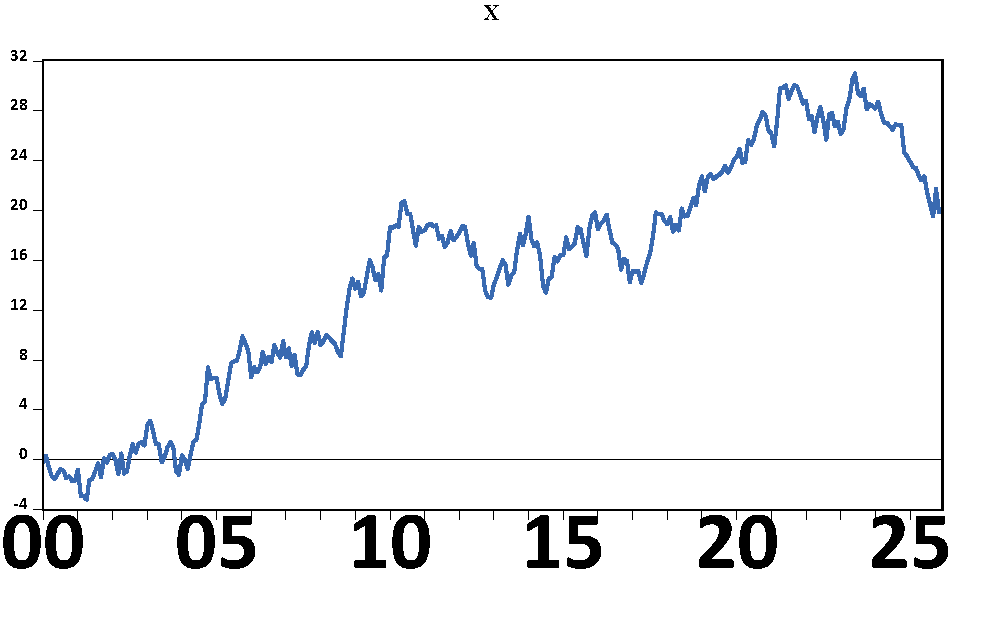
\includegraphics[width=0.45\textwidth]{test_engEviews_files/figure-latex//mychunk-grap2} }\newline\subfloat[A figure\label{fig:mychunk-3}]{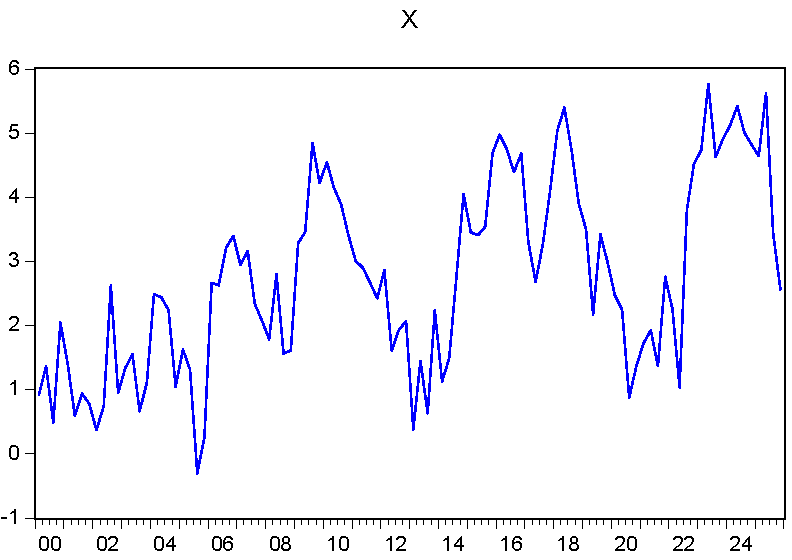
\includegraphics[width=0.45\textwidth]{test_engEviews_files/figure-latex//mychunk-grap} }

}

\caption{somefigure}\label{fig:mychunk}
\end{figure}

\begin{verbatim}
##        aic  df     coefs       dw        f    fprob       hq      logl
## 1 5.282974 102 -3.497069 0.104191 9.228703 0.003026 5.303577 -272.7147
## 2       NA  NA -0.154079       NA       NA       NA       NA        NA
##     meandep ncoef      pval       r2   rbar2 regobs  schwarz    sddep       se
## 1 -5.874184     2 0.0000777 0.082971 0.07398    104 5.333828 3.495431 3.363651
## 2        NA    NA 0.0030260       NA      NA     NA       NA       NA       NA
##        ssr  stderrs    tstats
## 1 1154.043 0.849166 -4.118237
## 2       NA 0.050719 -3.037878
\end{verbatim}

\begin{verbatim}
##        aic  df     coefs      dw        f    fprob       hq      logl  meandep
## 1 6.745148 102  4.050244 0.05466 29.21134 4.28e-07 6.765751 -348.7477 6.747683
## 2       NA  NA -1.318425      NA       NA       NA       NA        NA       NA
##   ncoef     pval       r2    rbar2 regobs  schwarz    sddep       se      ssr
## 1     2 5.95e-06 0.222628 0.215007    104 6.796002 7.886513 6.987437 4980.077
## 2    NA 4.28e-07       NA       NA     NA       NA       NA       NA       NA
##    stderrs    tstats
## 1 0.847674  4.778067
## 2 0.243938 -5.404752
\end{verbatim}

\begin{verbatim}
##         date         x           y          z
## 1 2000-01-01 0.2833776  0.41325243 -0.5082583
## 2 2000-04-01 1.3905559  0.05601737 -1.0322353
## 3 2000-07-01 1.6186456 -0.54610002 -0.3454605
## 4 2000-10-01 1.3899275  0.15314155 -1.4400351
## 5 2001-01-01 2.2350646  0.39452281 -1.8614388
## 6 2001-04-01 3.1352239  2.37738292 -1.4341431
\end{verbatim}

\hypertarget{r-plots}{%
\section{R plots}\label{r-plots}}

\begin{verbatim}
## NULL
\end{verbatim}

\begin{verbatim}
## [1] "asis"
\end{verbatim}

\begin{figure}[h]

{\centering 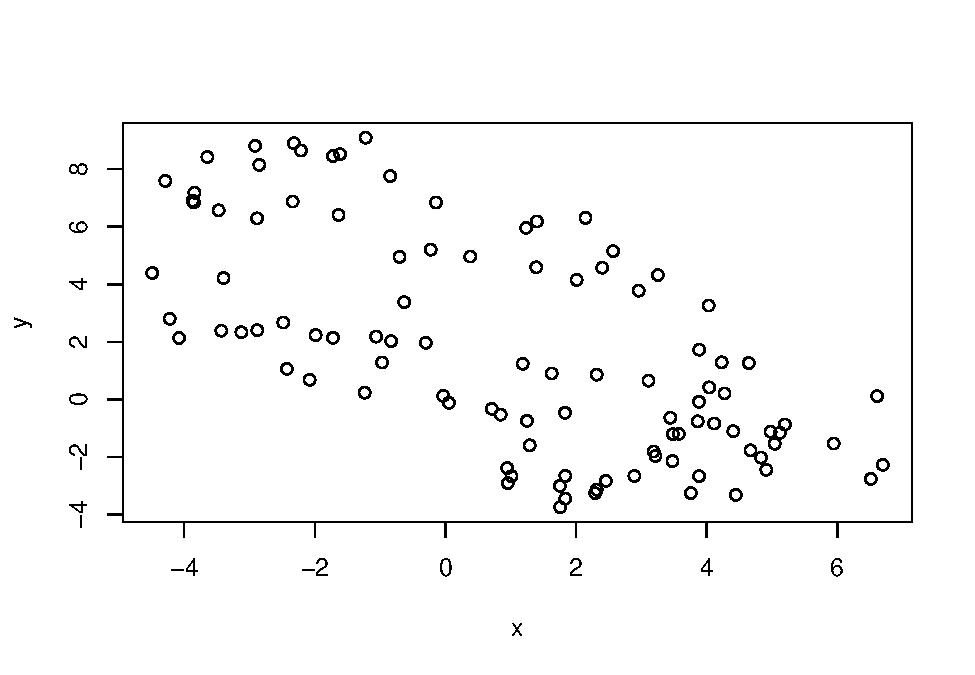
\includegraphics[width=0.45\textwidth]{test_engEviews_files/figure-latex/labe-1} 

}

\caption{another fig}\label{fig:labe}
\end{figure}

\begin{center}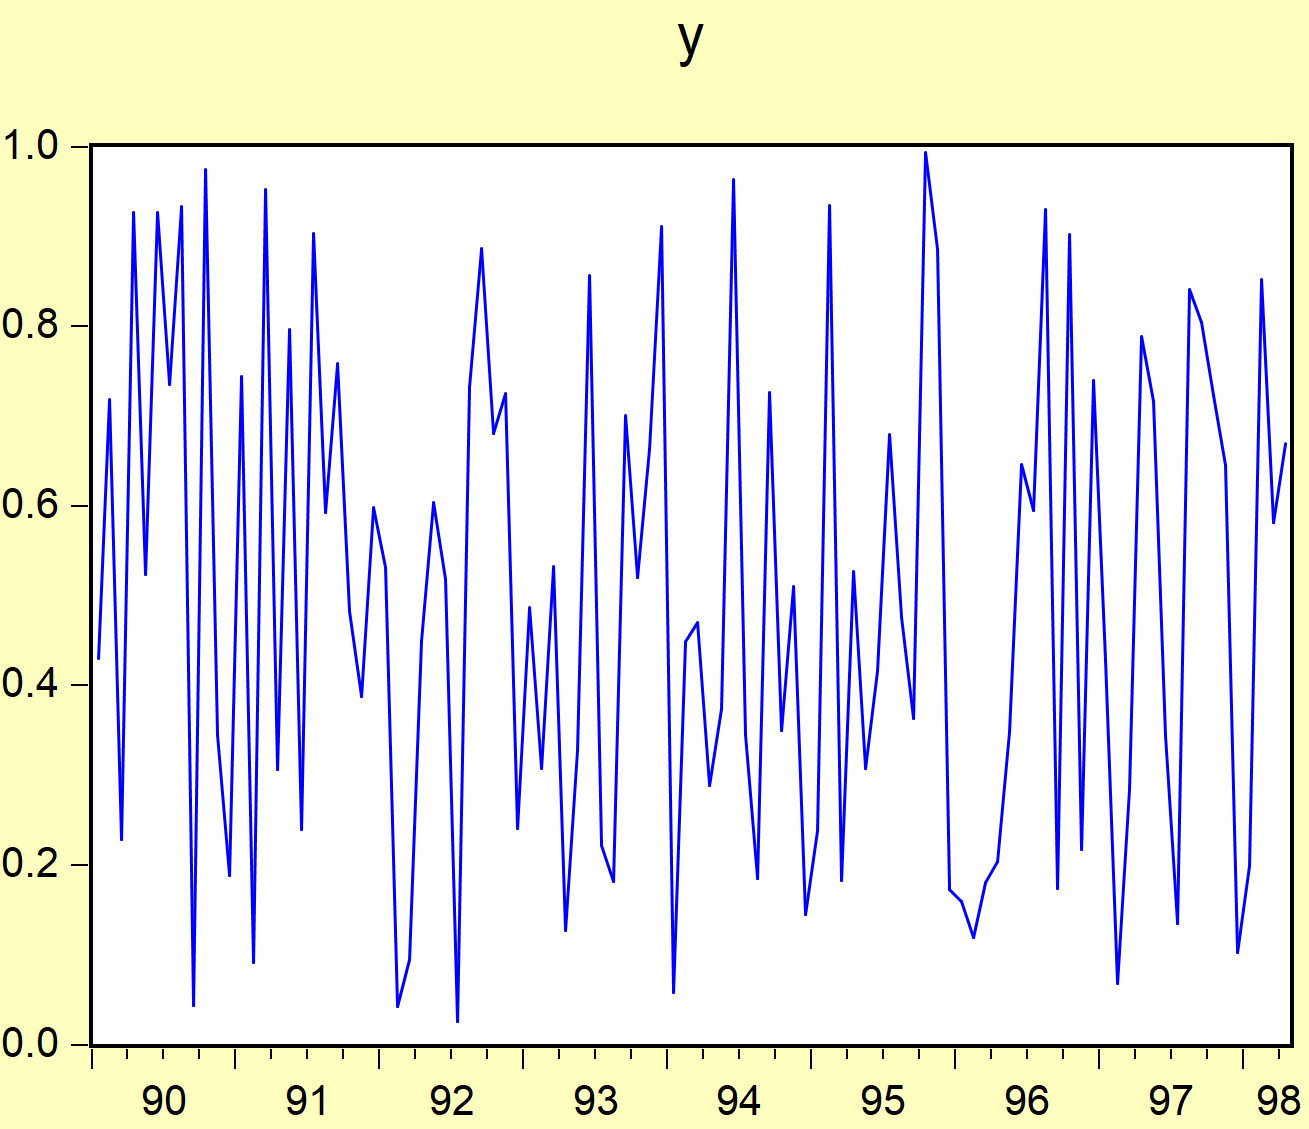
\includegraphics[width=0.45\textwidth]{test_engEviews_files/figure-latex//eview-graph-y} \end{center}

\begin{center}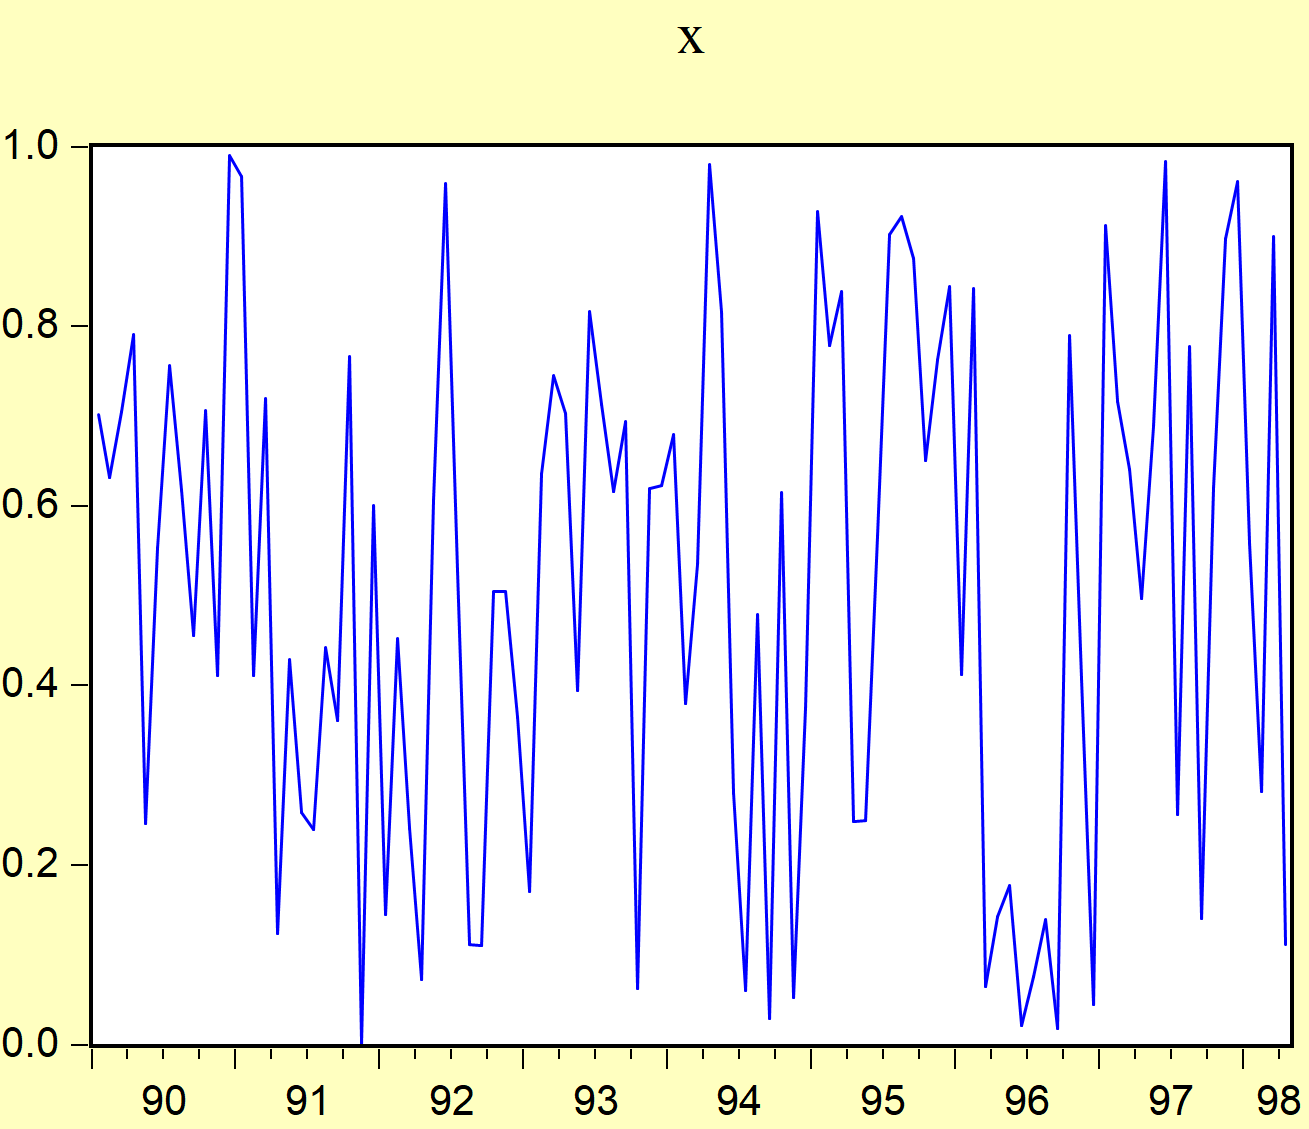
\includegraphics[width=0.45\textwidth]{test_engEviews_files/figure-latex//eview-graph-x} \end{center}

\begin{verbatim}
##         date          x          y         z
## 1 2001-01-01 -0.1752777 -0.8095509 -1.723300
## 2 2001-01-02 -2.0590310 -0.3201809 -2.492425
## 3 2001-01-03 -3.8612069 -0.8271296 -2.088396
## 4 2001-01-04 -2.4486016 -1.4653937 -3.378882
## 5 2001-01-05 -2.0373300 -1.5978963 -2.466871
## 6 2001-01-06 -3.5206709 -1.3343573 -1.249703
\end{verbatim}

\begin{center}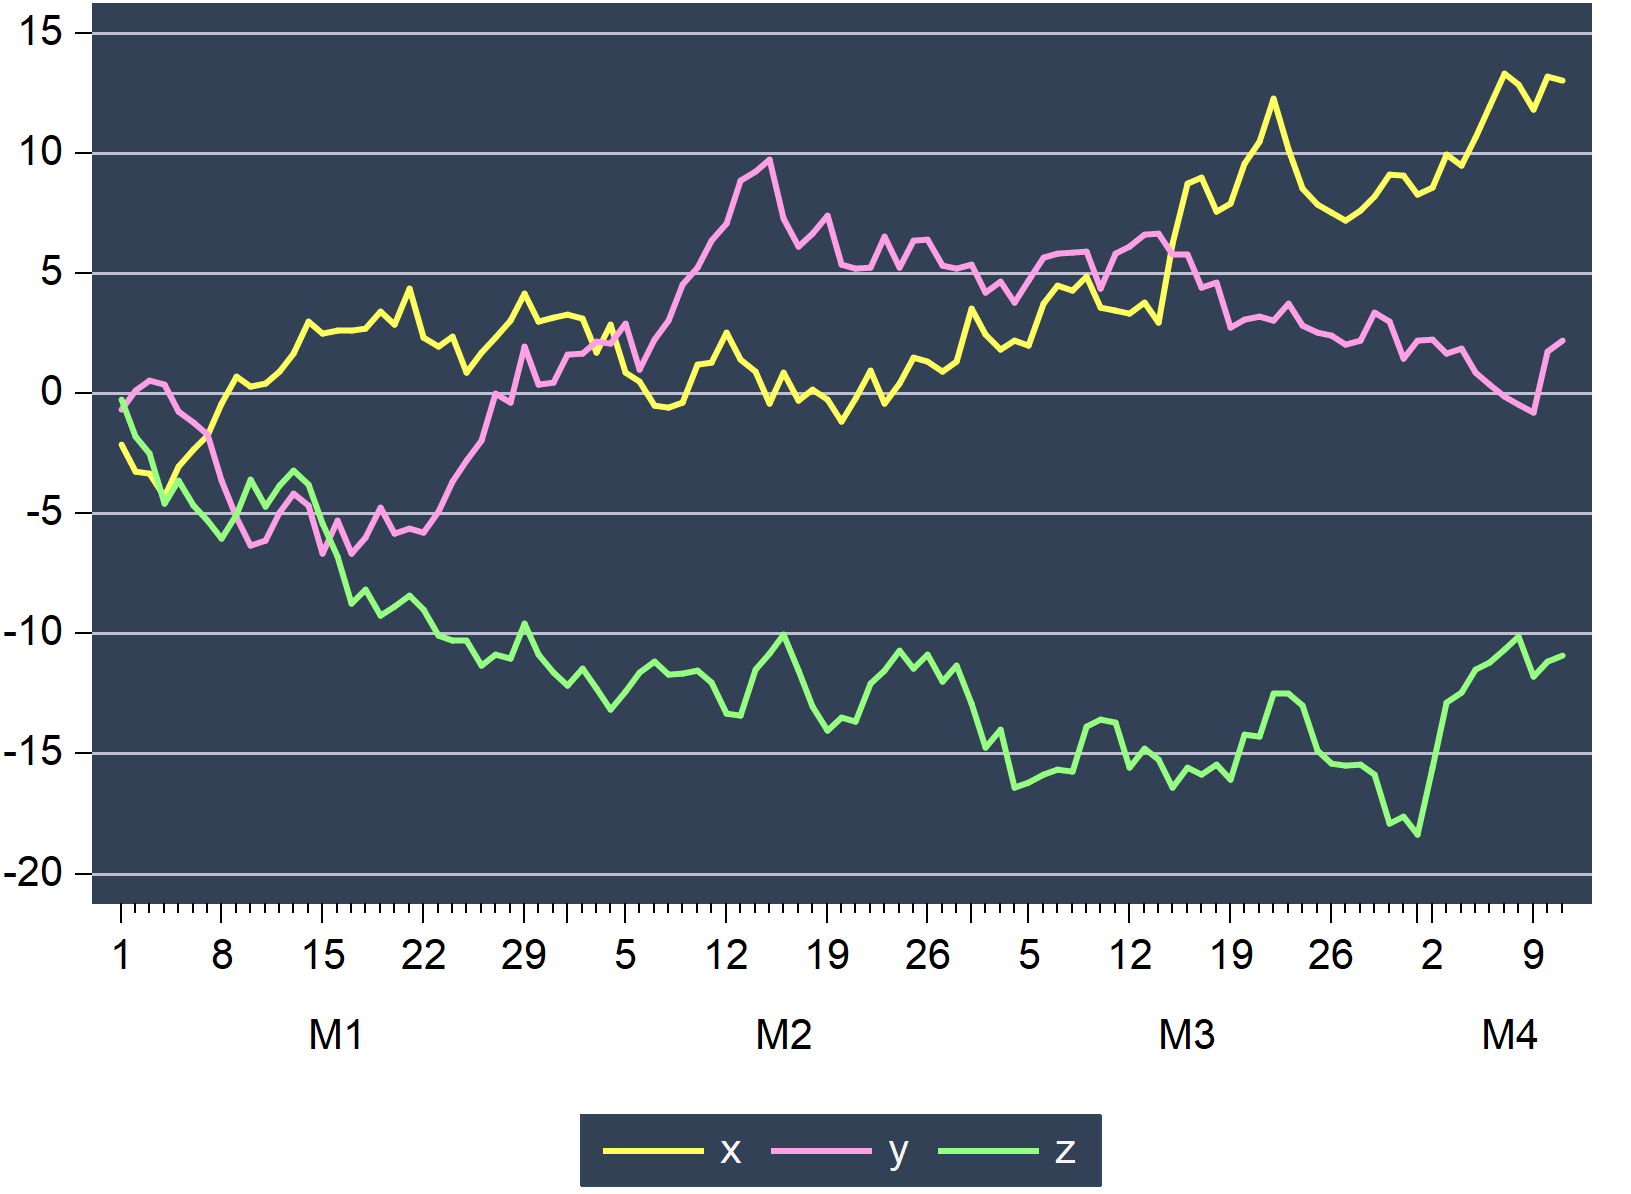
\includegraphics[width=0.45\textwidth]{test_engEviews_files/figure-latex//rwalk-xyz} \end{center}

\end{document}
